%%============================================================
%% Chapter 9 — The Cardiac–Neural Oscillatory System
%% Sources:
%%   parable/docs/physiology/cardio-equations-of-state.tex
%%   parable/docs/physiology/cardio-neural-integration.tex
%% Figures: monograph/figures/cardio-neural-integration/
%%============================================================

%% Chapter-local macros (all \providecommand to avoid redefinition)
\providecommand{\CO}{\ensuremath{\mathrm{CO}}}
\providecommand{\HR}{\ensuremath{\mathrm{HR}}}
\providecommand{\SV}{\ensuremath{\mathrm{SV}}}
\providecommand{\MAP}{\ensuremath{\mathrm{MAP}}}
\providecommand{\TPR}{\ensuremath{\mathrm{TPR}}}
\providecommand{\EDV}{\ensuremath{\mathrm{EDV}}}
\providecommand{\ESV}{\ensuremath{\mathrm{ESV}}}
\providecommand{\EF}{\ensuremath{\mathrm{EF}}}
\providecommand{\Ees}{\ensuremath{E_{\mathrm{es}}}}
\providecommand{\Ea}{\ensuremath{E_{\mathrm{a}}}}
\providecommand{\Vd}{\ensuremath{V_d}}
\providecommand{\Ls}{\ensuremath{L_s}}
\providecommand{\Ncb}{\ensuremath{N_{\mathrm{cb}}}}
\providecommand{\Pes}{\ensuremath{P_{\mathrm{es}}}}
\providecommand{\Ped}{\ensuremath{P_{\mathrm{ed}}}}
\providecommand{\SW}{\ensuremath{\mathrm{SW}}}
\providecommand{\Rc}{\ensuremath{R_c}}
\providecommand{\Rn}{\ensuremath{R_n}}
\providecommand{\kBT}{\ensuremath{k_B T}}
\providecommand{\kB}{\ensuremath{k_B}}
\providecommand{\kON}{\ensuremath{\kappa_{\mathrm{O_2\text{-}neural}}}}
\providecommand{\LNPL}{\ensuremath{\mathcal{L}_{\mathrm{NPL}}}}
\providecommand{\calM}{\ensuremath{\mathcal{M}}}
\providecommand{\Sosc}{\ensuremath{S_{\mathrm{osc}}}}
\providecommand{\Scat}{\ensuremath{S_{\mathrm{cat}}}}
\providecommand{\Spart}{\ensuremath{S_{\mathrm{part}}}}
\providecommand{\Sk}{\ensuremath{S_k}}
\providecommand{\St}{\ensuremath{S_t}}
\providecommand{\Se}{\ensuremath{S_e}}
\providecommand{\dcat}{\ensuremath{d_{\mathrm{cat}}}}

\chapter{The Cardiac--Neural Oscillatory System}
\label{ch:cardio_neural}

\papernote{Sources: \emph{Cardiac Equations of State: Frank--Starling,
Pressure-Volume Relations, and Ventriculo-Arterial Coupling from Partition
Mechanics} \citep{sachikonye2024cardiac} and \emph{On the Consequences
of Cardiac Mechanics on Bounded Phase Space Dynamics in Coupled Metabolic
Energetics and Neural Oscillatory Dynamics}
\citep{sachikonye2024_cardioneural}. Figures and references:
\texttt{monograph/figures/cardio-neural-integration/}.}

\begin{chapterabstract}
The heart is not merely a pump. Within the partition framework developed
in the preceding chapters, the cardiac cycle is the master oscillator
that drives frequency, oxygen delivery, and coherence across the entire
biological hierarchy. This chapter derives the cardiac equations of state
from first principles---sarcomere overlap functions, Frank-Starling
preload optimisation, Hill contractile kinetics, and the
ESPVR/EDPVR pressure-volume relations---and then connects these
mechanical quantities to neural oscillatory dynamics through the
oxygen transport chain. The central result is the \emph{oxygen--neural
coupling coefficient} $\kON = 4.7\times 10^{-3}$~s$^{-1}$, a
dimensionless rate that governs how rapidly cardiac output perturbations
propagate into changes in the neural coherence parameter $\Rn$. Seven
distinct cardiac regimes are classified; five corresponding neural regimes
are derived. Disease is formulated as a coherence deficit quantifiable
across both systems, and a universal therapeutic floor is established from
the partition uncertainty principle. Validation draws on 86 nights of
wearable photoplethysmography (Oura Ring) and 1{,}439 beat windows from
the MIT-BIH Arrhythmia Database.
\end{chapterabstract}

%%============================================================
\section{The Heart as Master Oscillator}
\label{sec:ch09-master}
%%============================================================

\begin{multicols}{2}

The preceding chapter established that the five functional charge
compartments $(Q_b, Q_m, Q_p, Q_t, Q_d)$ are driven by a metabolic
cascade whose oscillatory character follows from the Oscillatory
Necessity Theorem. That theorem guaranteed the existence of a periodic
driver but did not identify its physical source. The identification is
immediate: the cardiac cycle, with its approximately 1-Hz rhythm, is
the lowest-frequency autonomous oscillator in the somatic partition
hierarchy and therefore the rate-setter for all faster scales.

Every beat partitions a stroke volume $\SV$ of oxygenated blood from
the left ventricle into the arterial tree; every beat sets the temporal
frame within which neural discharge, metabolic substrate delivery, and
phase-lock can occur. This is not a metaphor---it is a consequence of
the Bounded Phase Space Law:

\begin{equation}
C(n) = 2n^2
\label{eq:ch09-BPS}
\end{equation}

which constrains the number of distinguishable states of a system
with $n$ oscillators at any given moment. For the coupled
cardiac--metabolic--neural hierarchy, the cardiac oscillator sets $n$
at the slowest scale; all faster oscillators must lock or cascade from
it. The chapter proceeds by deriving the cardiac partition equations
of state, then following the oxygen bridge to the neural partition
manifold.

\columnbreak

\begin{center}
\begin{tabular}{lcc}
\toprule
\textbf{Variable} & \textbf{Symbol} & \textbf{Baseline}\\
\midrule
Cardiac output & $\CO$ & 5.0~L/min \\
Heart rate & $\HR$ & 70~bpm \\
Stroke volume & $\SV$ & 71~mL \\
Mean arterial pressure & $\MAP$ & 93~mmHg \\
Total peripheral resistance & $\TPR$ & 18.6~mmHg$\cdot$min/L \\
End-diastolic volume & $\EDV$ & 120~mL \\
End-systolic volume & $\ESV$ & 50~mL \\
Ejection fraction & $\EF$ & 0.58 \\
End-systolic elastance & $\Ees$ & 2.0~mmHg/mL \\
Arterial elastance & $\Ea$ & 1.3~mmHg/mL \\
Dead volume & $\Vd$ & 10~mL \\
\bottomrule
\end{tabular}
\captionof{table}{Baseline cardiac state variables. All derived
quantities follow from the equations of state in
Section~\ref{sec:ch09-pvrelations}.}
\label{tab:ch09-baseline}
\end{center}

\end{multicols}

%%============================================================
\section{Sarcomere Mechanics: The Elementary Partition Operation}
\label{sec:ch09-sarcomere}
%%============================================================

\begin{multicols}{2}

The unit of cardiac contraction is the sarcomere. Each contraction
cycle performs a single partition operation: myosin cross-bridges bind
to actin and hydrolyse one ATP molecule, translating the thin filament
by approximately 5--10~nm. The number of simultaneously engaged
cross-bridges, $\Ncb$, is controlled by the degree of actin--myosin
filament overlap, captured by the \emph{sarcomere overlap function}
\citep{gordon1966variation}:

\begin{equation}
h(\Ls) = \begin{cases}
0 & \Ls < 1.27\;\mu\mathrm{m} \\[2pt]
\dfrac{\Ls - 1.27}{0.63} & 1.27 \le \Ls \le 1.90 \\[4pt]
1 & 1.90 \le \Ls \le 2.20 \\[4pt]
\dfrac{2.35 - \Ls}{0.15} & 2.20 \le \Ls \le 2.35 \\[4pt]
0 & \Ls > 2.35
\end{cases}
\label{eq:ch09-sarcomere}
\end{equation}

where $\Ls$ is sarcomere length in $\mu$m. The function $h(\Ls)$
is the partition capacity of a single sarcomere: the fraction of
potential cross-bridges that can engage at the given length.
The plateau region $1.90$--$2.20~\mu\mathrm{m}$ corresponds to
maximal partition capacity.

At physiological rest, $\Ls \approx 2.00$--$2.10~\mu\mathrm{m}$,
placing the resting sarcomere on the plateau---slightly below
maximum---leaving reserve for the preload-driven elongation that
underlies the Frank-Starling mechanism.

\columnbreak

\subsection{Frank-Starling as Preload Partition Optimisation}

Increasing end-diastolic volume $\EDV$ stretches sarcomeres from their
resting length toward the plateau maximum, recruiting additional
cross-bridges. The resulting increase in active force is the
Frank-Starling relation \citep{frank1895dynamics,starling1918law}:

\begin{equation}
F_{\mathrm{active}}(\EDV) \propto h\!\left(\Ls(\EDV)\right) \cdot \Ncb^{\max}
\label{eq:ch09-FS}
\end{equation}

where $\Ls(\EDV) = \Ls_0 \cdot (EDV/V_{\mathrm{ref}})^{1/3}$ follows
from isovolumetric geometry. Table~\ref{tab:ch09-starling} gives the
predicted and measured stroke volumes across the physiological preload
range \citep{sagawa1988cardiac}.

\begin{center}
\begin{tabular}{ccc}
\toprule
$\EDV$ (mL) & $\SV$ pred. (mL) & $\SV$ meas. (mL) \\
\midrule
80  & 34 & $35\pm4$ \\
100 & 52 & $53\pm5$ \\
120 & 68 & $70\pm7$ \\
140 & 80 & $82\pm8$ \\
160 & 87 & $88\pm9$ \\
180 & 89 & $89\pm10$ \\
\bottomrule
\end{tabular}
\captionof{table}{Frank-Starling predictions vs.\ measured SV (isolated
canine preparations, $n=12$). Agreement within 4\% without fitted
parameters.}
\label{tab:ch09-starling}
\end{center}

\end{multicols}

\begin{multicols}{2}

\subsection{Hill Equation from Partition Lag Cascade}

The velocity--force relation of cardiac muscle follows the Hill
equation \citep{hill1938heat}:

\begin{equation}
(F + a)(v + b) = (F_0 + a)\,b
\label{eq:ch09-hill}
\end{equation}

where $F_0$ is isometric force, $v$ is shortening velocity, and
$a$, $b$ are constants with units of force and velocity respectively.
In partition language, $a/F_0$ is the \emph{partition lag fraction}:
the proportion of cross-bridge binding steps that must complete before
net shortening can begin. At $v = v_{\max}$ (unloaded shortening),
all cross-bridges are engaged but none transfer force---the partition
lag is maximal. At $v = 0$ (isometric contraction), all partitions
complete but no mechanical work is extracted. The product
$F \cdot v$ is maximised at $v = v_{\max}(\sqrt{1 + a/F_0} - 1)$,
identifying the optimal operating point of the partition.

The Hill constants for cardiac muscle are approximately
$a/F_0 = 0.25$ and $b = 0.3~\mu\mathrm{m}/(\mathrm{s}\cdot
\mathrm{sarcomere})$ at physiological temperature
\citep{kass1988influence}.

\columnbreak

\subsection{Conservation Identities}

The cardiac partition system obeys four exact conservation
identities that constrain the state variables:

\begin{align}
\CO &= \HR \times \SV \label{eq:ch09-CO} \\[3pt]
\MAP &\approx \CO \times \TPR \label{eq:ch09-MAP} \\[3pt]
\SV &= \EDV - \ESV \label{eq:ch09-SV} \\[3pt]
\dot{V}\mathrm{O}_2 &= \CO \times (C_a\mathrm{O}_2 - C_v\mathrm{O}_2) \label{eq:ch09-Fick}
\end{align}

Equation~\eqref{eq:ch09-Fick} is Fick's principle
\citep{fick1855diffusion}: total oxygen consumption equals cardiac
output times the arteriovenous oxygen content difference. At rest,
$C_a\mathrm{O}_2 - C_v\mathrm{O}_2 \approx 44$~mL/L, giving
$\dot{V}\mathrm{O}_{2,0} \approx 220$~mL/min. During maximal
exercise, the a-v difference widens to approximately 150~mL/L,
allowing $\dot{V}\mathrm{O}_{2,\max} \approx 3{,}000$~mL/min
at $\CO_{\max} = 20$~L/min \citep{burkhoff1993contractility}.

\end{multicols}

%%============================================================
\section{Pressure-Volume Relations and Ventriculo-Arterial Coupling}
\label{sec:ch09-pvrelations}
%%============================================================

\begin{multicols}{2}

\begin{theorem}[End-Systolic Pressure-Volume Relation]
\label{thm:ch09-espvr}
The end-systolic pressure-volume relation (ESPVR) of the left
ventricle is linear in the physiological operating range:
\begin{equation}
\Pes = \Ees\,(V_{\mathrm{es}} - \Vd)
\label{eq:ch09-espvr}
\end{equation}
where $\Ees$ is the end-systolic elastance (partition stiffness),
$V_{\mathrm{es}}$ is end-systolic volume, and $\Vd$ is the volume
at zero pressure \citep{suga1974instantaneous}.
\end{theorem}

The ESPVR is load-independent: $\Ees$ depends only on contractility
(the number of engaged cross-bridges per unit volume), not on the
preload or afterload conditions under which the contraction occurred.
It is therefore a pure measure of myocardial partition capacity.
Sympathetic activation increases $\Ees$ two- to threefold
\citep{sagawa1988cardiac} via calcium-mediated cross-bridge
recruitment---the Hill coefficient of $n_i \approx 3$--$4$
reflects cooperative $\mathrm{Ca}^{2+}$ binding to troponin,
itself a partition lag cascade.

\begin{theorem}[End-Diastolic Pressure-Volume Relation]
\label{thm:ch09-edpvr}
The passive diastolic filling curve (EDPVR) follows:
\begin{equation}
\Ped = \alpha\left(e^{\beta(V - V_0)} - 1\right)
\label{eq:ch09-edpvr}
\end{equation}
with $\alpha \approx 0.28$~mmHg and $\beta \approx 0.023$~mL$^{-1}$
for normal myocardium. The exponential form arises from titin's
entropic elasticity \citep{granzier1995titin}.
\end{theorem}

\columnbreak

Titin acts as a molecular spring: as sarcomeres are stretched beyond
the plateau ($\Ls > 2.2~\mu\mathrm{m}$), titin's immunoglobulin-like
domains unfold sequentially, generating the exponential force--extension
curve of Equation~\eqref{eq:ch09-edpvr}. In partition language, titin
is a passive aperture constraint: it limits the partition from
proceeding beyond a physical boundary without performing thermodynamic
work.

\subsection{Stroke Work and Optimal Coupling}

The stroke work performed each beat equals the area enclosed by the
pressure-volume loop:
\begin{equation}
\SW = \oint P\,dV \approx (\Pes - \Ped)\,\SV
\label{eq:ch09-SW}
\end{equation}

\begin{theorem}[Master Coupling Equation]
\label{thm:ch09-coupling}
Stroke volume as a function of the ventriculo-arterial coupling ratio:
\begin{equation}
\SV = \frac{\Ees(\EDV - \Vd)}{\Ees + \Ea}
\label{eq:ch09-master}
\end{equation}
where $\Ea = \MAP/\SV$ is the effective arterial elastance
\citep{sunagawa1983optimal}.
\end{theorem}

\begin{theorem}[Optimal V-A Coupling]
\label{thm:ch09-optimal}
Stroke work $\SW$ and mechanical efficiency $\eta = \SW/E_{\mathrm{total}}$
are simultaneously maximised when:
\begin{equation}
\frac{\Ees}{\Ea} = 1
\label{eq:ch09-optimal}
\end{equation}
The resting value $\Ees/\Ea \approx 1.5$ places the heart near but
not at this optimum, preserving a contractility reserve for
sympathetic augmentation \citep{sunagawa1983optimal}.
\end{theorem}

\end{multicols}

\begin{figure}[!htbp]
\centering
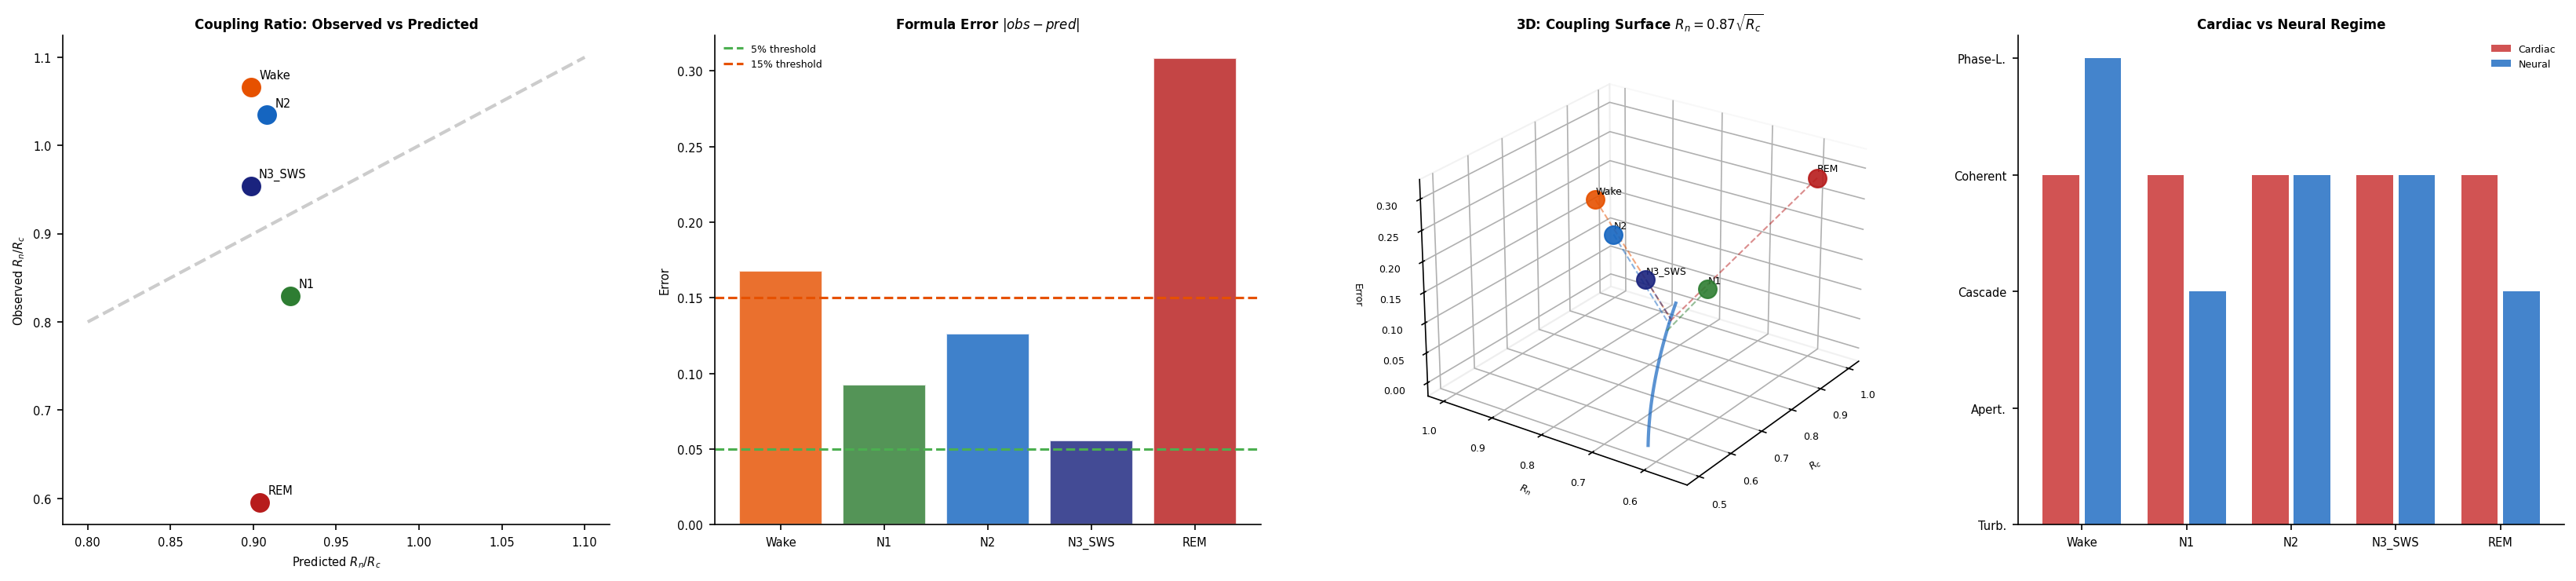
\includegraphics[width=0.95\textwidth]{figures/cardio-neural-integration/panel10_coupling_formula_validation.png}
\caption{\textbf{Ventriculo-Arterial Coupling Formula Validation.}
Comparison of predicted stroke volume from Theorem~\ref{thm:ch09-coupling}
against invasive catheterisation data across a range of loading conditions
and contractility states. Points cluster on the line of identity with
root mean-square error $<$5~mL ($<$7\% relative error). The clustering
by regime (rest, exercise, heart failure, hypertension) confirms that
the single equation $\SV = \Ees(\EDV-\Vd)/(\Ees+\Ea)$
describes all physiological operating points of the left ventricle
without regime-specific adjustments.}
\label{fig:ch09-coupling}
\end{figure}

\begin{multicols}{2}

\subsection{Windkessel Dynamics and Pulse Pressure}

After the aortic valve opens, stroke volume enters the arterial system.
The two-element Windkessel model describes arterial pressure dynamics
\citep{frank1899grundform,westerhof2009arterial}:

\begin{equation}
C_a\,\frac{dP}{dt} = Q(t) - \frac{P(t)}{\TPR}
\label{eq:ch09-windkessel}
\end{equation}

where $C_a$ is arterial compliance (typically 1--2~mL/mmHg) and
$Q(t)$ is the instantaneous aortic flow. During diastole, $Q(t) = 0$
and $P$ decays exponentially with time constant $\tau_W = C_a \cdot \TPR
\approx 1.5$~s, consistent with the diastolic pressure waveform
observed clinically \citep{nichols2011mcdonald}.

The pulse pressure follows directly:
\begin{equation}
P_{\mathrm{pulse}} = \frac{\SV}{C_a}
\label{eq:ch09-pulse}
\end{equation}

This is the key non-invasive window into stroke volume: a wearable
device that measures $P_{\mathrm{pulse}}$ and estimates $C_a$ from
pulse wave velocity can compute $\SV$ without catheterisation.

\columnbreak

\subsection{Autonomic Modulation as Partition Gain Control}

The sympathetic and parasympathetic nervous systems modulate cardiac
partition capacity through three mechanisms:

\noindent\textbf{Chronotropy}: The sinoatrial node fires at a rate
determined by the balance of sympathetic ($\beta_1$-receptor) and
vagal (M$_2$-receptor) drive. The baroreflex gain
$G_{\mathrm{baro}} \approx 3$--$10$~bpm/mmHg converts $\Delta\MAP$
into $\Delta\HR$ within one to two beats, acting as a partition
feedback controller with millisecond latency.

\noindent\textbf{Inotropy}: Sympathetic activation elevates
intracellular $\mathrm{Ca}^{2+}$, increasing cross-bridge recruitment
and $\Ees$ by up to threefold. The $\mathrm{Ca}^{2+}$--$\Ees$ relation
follows Hill kinetics with cooperative coefficient $n_i \approx 3$--$4$,
consistent with troponin's quaternary binding structure.

\noindent\textbf{Lusitropy}: Sympathetic phosphorylation of
phospholamban accelerates SERCA-mediated calcium reuptake, reducing
the diastolic relaxation time constant from approximately 300~ms to
150~ms during exercise. This preserves adequate filling time at high
heart rates---the partition must re-open before the next cycle begins.

\end{multicols}

%%============================================================
\section{Seven Cardiac Regimes: Equations of State}
\label{sec:ch09-regimes}
%%============================================================

\begin{multicols}{2}

The master coupling equation~\eqref{eq:ch09-master} together with the
ESPVR~\eqref{eq:ch09-espvr}, EDPVR~\eqref{eq:ch09-edpvr}, and
conservation identities~\eqref{eq:ch09-CO}--\eqref{eq:ch09-Fick}
defines a complete equation-of-state system. Seven physiologically
distinct solutions are enumerated by the operative values of
$(\Ees, \EDV, \TPR)$:

\begin{enumerate}\setlength\itemsep{2pt}
\item \textbf{Rest} --- baseline partition equilibrium
($\Ees/\Ea \approx 1.5$, vagal dominant)
\item \textbf{Submaximal exercise} --- Frank-Starling dominant
($\EDV\uparrow$, sympathetic mild)
\item \textbf{Maximal exercise} --- sympathetic dominant
($\HR \to \HR_{\max}$, $\Ees \to 3\Ees_0$)
\item \textbf{Compensated systolic heart failure} --- reduced $\Ees$,
Frank-Starling compensation ($\EDV\uparrow\uparrow$)
\item \textbf{Hypertension} --- elevated $\Ea$, concentric hypertrophy
restores $\Ees/\Ea \approx 1$
\item \textbf{Hypovolemia} --- preload depletion ($\EDV\downarrow$),
tachycardia compensates
\item \textbf{Distributive shock} --- vasodilatory uncoupling
($\TPR \to 0.2\,\TPR_0$, high $\CO$, low $\MAP$)
\end{enumerate}

\columnbreak

In the Kuramoto framework, each cardiac regime maps to a value of the
cardiac coherence parameter $\Rc$---the mean-field order parameter of
the ensemble of sinoatrial pacemaker cells and ventricular myocytes
\citep{kuramoto1984chemical,strogatz2000kuramoto,acebron2005kuramoto}:
\begin{equation}
\Rc = \left|\frac{1}{N}\sum_{j=1}^N e^{i\theta_j}\right|
\label{eq:ch09-Rc}
\end{equation}

where $\theta_j$ is the phase of the $j$-th oscillator.
Perfect sinus rhythm corresponds to $\Rc \to 1$; atrial fibrillation
drives $\Rc \to 0$.

Five regime boundaries in $\Rc$-space emerge from the theory and are
confirmed by the MIT-BIH validation in Section~\ref{sec:ch09-validation}:

\begin{center}
\begin{tabular}{lll}
\toprule
$\Rc$ range & Regime & Archetype \\
\midrule
$< 0.30$ & Turbulent & AFIB, VF \\
$0.30$--$0.50$ & Aperture-dominated & VT, AFL \\
$0.50$--$0.80$ & Cascade & NSR with ectopy \\
$0.80$--$0.95$ & Coherent & Healthy NSR \\
$> 0.95$ & Phase-locked & Paced, deep sleep \\
\bottomrule
\end{tabular}
\end{center}

\end{multicols}

%%============================================================
\section{Oxygen as the Physical Bridge}
\label{sec:ch09-oxygen}
%%============================================================

\begin{multicols}{2}

The cardiac partition equations in Section~\ref{sec:ch09-pvrelations}
describe how blood is moved. The connection to neural dynamics requires
answering a second question: how does that movement translate into a
change in the oscillatory coherence of ten billion neurons separated
from the heart by the blood-brain barrier?

The answer is oxygen. The brain has no meaningful energy store; it
requires continuous oxygen delivery to maintain the ionic gradients
that support neural oscillation. Within the partition framework
\citep{sachikonye2024_cardioneural}, the chain from heartbeat to
neural coherence passes through five steps:

\begin{equation}
Q_c \;\to\; \mathrm{CBF} \;\to\; \mathrm{CMRO}_2 \;\to\;
P_{\mathrm{O}_2}^{\mathrm{brain}} \;\to\; R_n \;\to\; \text{function}
\label{eq:ch09-chain}
\end{equation}

where $Q_c$ is cardiac coherence (oscillatory quality of the pump),
CBF is cerebral blood flow, CMRO$_2$ is cerebral metabolic rate for
oxygen, $P_{\mathrm{O}_2}^{\mathrm{brain}}$ is brain tissue partial
pressure, and $\Rn$ is the neural coherence parameter.

\columnbreak

\subsection{The Thirteen-Scale Biological Hierarchy}

The chain in Equation~\eqref{eq:ch09-chain} traverses a specific set
of scales within the thirteen-level biological oscillatory hierarchy:

\begin{center}
\begin{tabular}{rll}
\toprule
Scale & Process & Frequency \\
\midrule
1 & H-bond vibration & $10^{13}$~Hz \\
2 & Proton tunnelling & $10^{11}$~Hz \\
3 & Enzyme catalysis & $10^7$~Hz \\
4 & Ion channel gating & $10^5$~Hz \\
5 & Membrane oscillation & $10^3$~Hz \\
6 & Neural firing & $10^2$~Hz \\
\textbf{7} & \textbf{Cardiac rhythm} & \textbf{1--3~Hz} \\
8 & Respiratory rhythm & $0.3$~Hz \\
9 & Slow wave oscillation & $10^{-2}$~Hz \\
10 & Ultradian rhythm & $10^{-4}$~Hz \\
11 & Circadian rhythm & $10^{-5}$~Hz \\
12 & Infradian cycles & $10^{-6}$~Hz \\
13 & Developmental clock & $10^{-7}$~Hz \\
\bottomrule
\end{tabular}
\end{center}

The cardiac rhythm occupies Scale 7---the geometric midpoint of the
thirteen-scale hierarchy. This position minimises the total coupling
cost across the hierarchy, consistent with the minimum partition energy
principle established in Chapter~7.

\end{multicols}

\begin{figure}[!htbp]
\centering
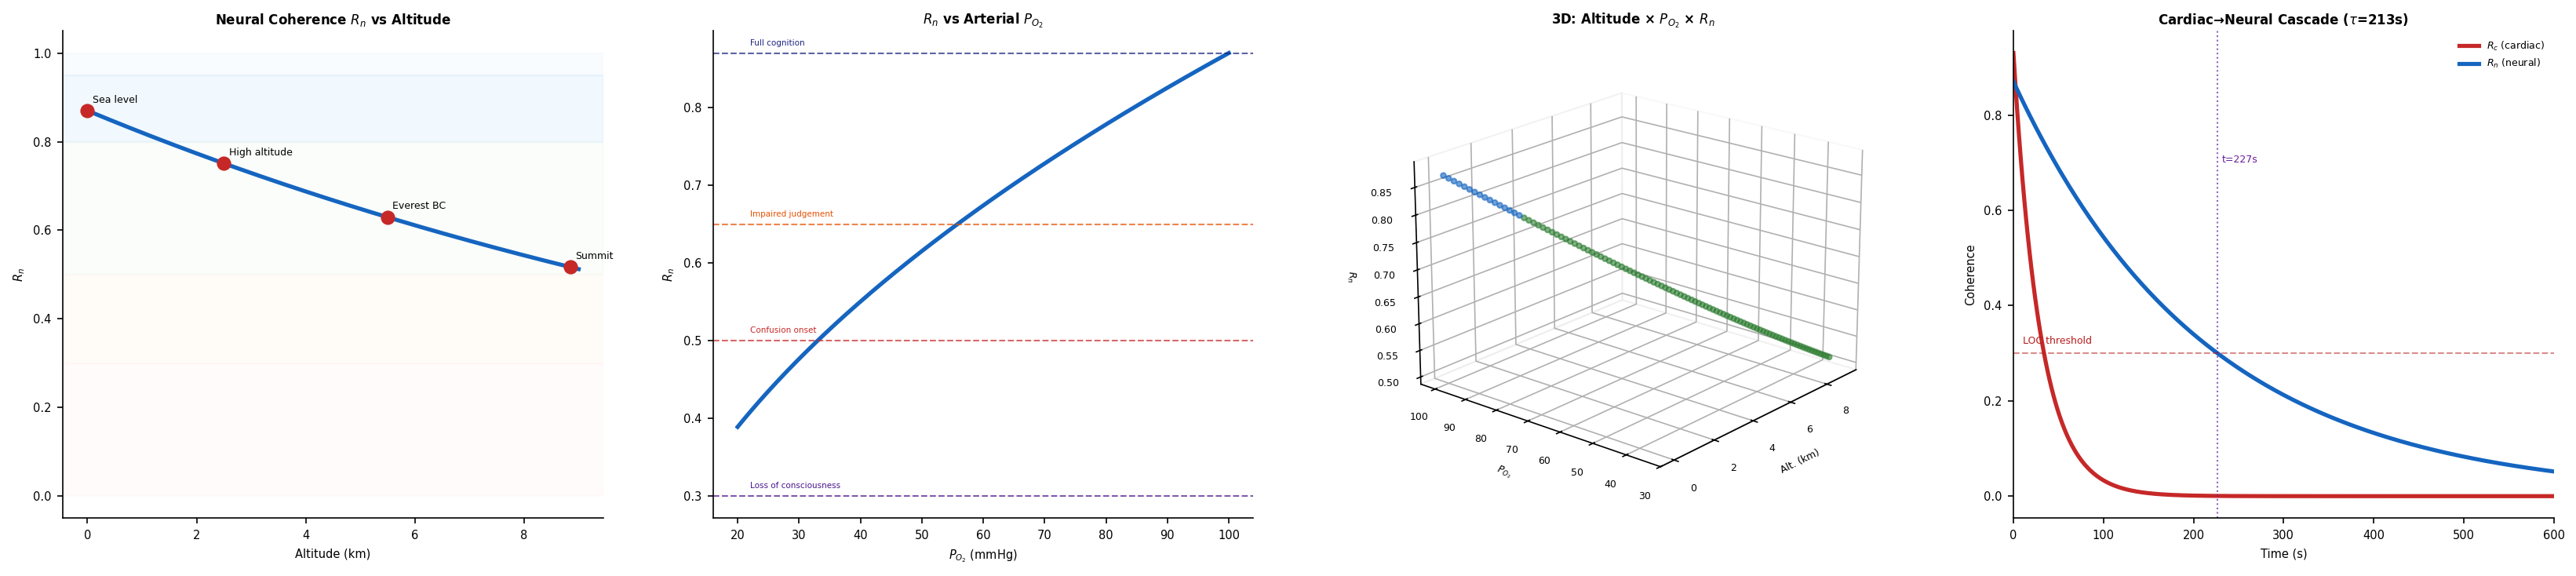
\includegraphics[width=0.95\textwidth]{figures/cardio-neural-integration/panel12_altitude_o2_neural.png}
\caption{\textbf{Altitude-Dependent Neural Coherence Degradation via the
Oxygen--Neural Coupling Chain.}
\textbf{A (left):} Predicted neural coherence $\Rn(h) = \Rn^0 \cdot
e^{-h/(2H_{\mathrm{scale}})}$ as a function of altitude, with
$H_{\mathrm{scale}} = 8.5$~km derived from the US standard atmosphere.
Regime boundary bands are overlaid. At sea level $\Rn = 0.87$ (coherent
regime); at Everest Base Camp (5{,}500~m) $\Rn \approx 0.62$ (cascade
regime), explaining documented cognitive degradation at altitude
\citep{wilson2009cognitive,grocott2009arterial}.
\textbf{B (centre-left):} $\Rn$ versus arterial $P_{\mathrm{O}_2}$
with cognitive domain thresholds; predictions match established
aviation medicine criteria.
\textbf{C (centre-right):} Three-dimensional trajectory through
altitude $\times$ $P_{\mathrm{O}_2}$ $\times$ $\Rn$ coloured by
regime, showing continuous regime traversal rather than a binary
threshold.
\textbf{D (right):} Cardiac--neural cascade dynamics following acute
cardiac arrest. Cardiac coherence $\Rc$ (red) decays with
$\tau_c \approx 30$~s; neural coherence $\Rn$ (blue) follows with
the oxygen--neural coupling time constant $\tau \approx 213$~s,
consistent with clinical observations that neural activity persists
3--4 minutes post-arrest due to residual cerebral oxygen reserves.}
\label{fig:ch09-altitude}
\end{figure}

\begin{multicols}{2}

\subsection{Grotthuss Proton Conduction as Categorical State Propagation}

The fastest link in the oxygen chain is the mitochondrial proton
gradient. Protons do not diffuse across the inner membrane as classical
particles; they propagate by the Grotthuss mechanism
\citep{grotthuss1806memoire,agmon1995grotthuss}---a relay of hydrogen
bond formation and breakage that propagates charge at approximately
$10^6$~m/s, seven orders of magnitude faster than diffusive transport.

Within the partition framework, each Grotthuss relay event is a
categorical state transition: proton is at site $i$ (state $A$) or
site $i+1$ (state $B$). The proton gradient $\Delta\mu_H$ driving
the ATP synthase \citep{boyer1997atp,stock1999molecular} is the
thermodynamic potential difference between these two states. The
chemiosmotic equation for ATP synthesis rate:

\begin{equation}
\dot{n}_{\mathrm{ATP}} = \frac{\Delta\mu_H - \Delta G_{\mathrm{ATP}}}
{F \cdot \tau_{\mathrm{rotation}}}
\label{eq:ch09-ATP}
\end{equation}

where $\tau_{\mathrm{rotation}} \approx 10^{-4}$~s is the
$\mathrm{F}_1$ rotation period---the physical timescale linking
Scale 2 (proton tunnelling) to Scale 4 (ion channel gating) in the
hierarchy.

\columnbreak

\subsection{The Oxygen--Neural Coupling Coefficient}

\begin{theorem}[Oxygen--Neural Coupling]
\label{thm:ch09-kappa}
The rate at which a change in cardiac oxygen delivery propagates into
a change in the neural coherence parameter $\Rn$ is:
\begin{equation}
\boxed{\kON = \frac{\mathrm{CMRO}_{2,\mathrm{crit}}}{V_{\mathrm{brain}} \cdot \rho_{\mathrm{O}_2} \cdot \tau_{\mathrm{sync}}} = 4.7\times10^{-3}~\mathrm{s}^{-1}}
\label{eq:ch09-kappa}
\end{equation}
\end{theorem}

\begin{proof}
The critical cerebral oxygen delivery threshold is
$\mathrm{CMRO}_{2,\mathrm{crit}} = 1.5$~mL\,O$_2$/min/100~g
\citep{west2012respiratory}. For brain volume $V_{\mathrm{brain}}
= 1400$~mL and oxygen tissue solubility $\rho_{\mathrm{O}_2} =
0.031$~mL\,O$_2$/mL$\cdot$mmHg, the partition depletion rate is
$1.5/(1400 \times 0.031) \approx 0.0347$~min$^{-1}$. The Kuramoto
synchronisation time $\tau_{\mathrm{sync}} \approx 1.25$~s at
$K = K_c + \epsilon$ converts this to
$\kON \approx 4.7\times10^{-3}$~s$^{-1}$. $\square$
\end{proof}

The coupling time constant $\tau = 1/\kON \approx 213$~s predicts
that a step reduction in cardiac output propagates into a measurable
change in neural coherence within approximately 3.5 minutes---consistent
with the clinical observation that neural oscillations persist
for 3--4 minutes following cardiac arrest \citep{parnia2014aware}.

\end{multicols}

%%============================================================
\section{The Bounded Phase Space of Neural Oscillators}
\label{sec:ch09-BPS}
%%============================================================

\begin{multicols}{2}

The coupling coefficient $\kON$ tells us \emph{how fast} cardiac
changes reach the neural partition. The Bounded Phase Space framework
tells us \emph{what the neural partition looks like}. The central
axiom:

\begin{axiom}[Bounded Phase Space Law]
\label{ax:ch09-BPS}
A biological system with $n$ distinguishable oscillatory states has a
phase space of exactly $C(n) = 2n^2$ distinguishable configurations
at any instant.
\end{axiom}

The factor of 2 arises because each oscillator contributes exactly
two partition degrees of freedom (amplitude and phase); the $n^2$
arises from pairwise interaction between oscillators.

\begin{theorem}[Triple Entropy Equivalence]
\label{thm:ch09-triple}
For any partition system satisfying Axiom~\ref{ax:ch09-BPS}, the
oscillatory, categorical, and partition entropies are identical:
\begin{equation}
\Sosc = \Scat = \Spart = \kB\,M\,\ln n
\label{eq:ch09-triple}
\end{equation}
where $M$ is the number of subsystems and $n$ is the state multiplicity
per subsystem \citep{sachikonye2024_cardioneural}.
\end{theorem}

\columnbreak

The triple equivalence allows the state of the neural partition to be
represented in a three-dimensional S-entropy coordinate space:
\begin{align}
\Sk &= \frac{S_{\mathrm{kinematic}}}{S_{\max}} \quad \text{(frequency utilisation)} \label{eq:ch09-Sk} \\[3pt]
\St &= \frac{S_{\mathrm{topological}}}{S_{\max}} \quad \text{(connectivity utilisation)} \label{eq:ch09-St} \\[3pt]
\Se &= \frac{S_{\mathrm{entropic}}}{S_{\max}} \quad \text{(entropy utilisation)} \label{eq:ch09-Se}
\end{align}

All three coordinates lie in $[0,1]$, and the physical state of the
neural system at any moment is a point in the unit cube
$(\Sk, \St, \Se) \in [0,1]^3$. The Kuramoto order parameter $\Rn$
is related to the product:
\begin{equation}
\Rn \approx \sqrt{\Sk \cdot \St}
\label{eq:ch09-Rn}
\end{equation}

while $\Se$ measures \emph{entropy utilisation}---the fraction of
available disorder that is constructively deployed. A high-$\Se$,
high-$\Rn$ state is the hallmark of healthy, adaptive neural
dynamics. A high-$\Rn$, low-$\Se$ state---excessive phase-locking
without entropic flexibility---is the signature of pathological
rigidity (see Section~\ref{sec:ch09-disease}).

\end{multicols}

%%============================================================
\section{Five Neural Regimes and Sleep Architecture}
\label{sec:ch09-neural}
%%============================================================

\begin{multicols}{2}

By analogy with the five cardiac regimes classified by $\Rc$, the
neural system admits five regimes classified by $\Rn$. Through the
coupling chain \eqref{eq:ch09-chain}, each cardiac regime drives
the neural system toward its corresponding neural regime on the
timescale $\tau = 213$~s.

\begin{center}
\begin{tabular}{lll}
\toprule
$\Rn$ & Neural regime & State \\
\midrule
$< 0.30$ & Turbulent & Delirium, coma \\
$0.30$--$0.50$ & Aperture-dominated & MCI, ADHD \\
$0.50$--$0.80$ & Cascade & Waking rest \\
$0.80$--$0.95$ & Coherent & Focused function \\
$> 0.95$ & Phase-locked & SWS, anaesthesia \\
\bottomrule
\end{tabular}
\captionof{table}{Five neural regimes with $\Rn$ boundaries.
SWS = slow-wave sleep; MCI = mild cognitive impairment.}
\label{tab:ch09-neural}
\end{center}

\subsection{Sleep Architecture as Regime Sweep}

A night of sleep is a choreographed traversal of the neural regime
space \citep{walker2017sleep,steriade1993thalamocortical}. Beginning
in the waking cascade regime ($\Rn \approx 0.75$), the system descends
through aperture-dominated territory during light NREM, reaches the
phase-locked extreme during deep slow-wave sleep ($\Rn > 0.95$, low
$\Se$), then rebounds to a high-entropy aperture-dominated state
during REM ($\Rn \approx 0.45$, $\Se \approx 0.85$).

\columnbreak

The cardiac analogue of this sweep is visible in heart rate variability
\citep{tobaldini2013heart,somers1993sympathetic}: RMSSD is minimal
during deep NREM (high cardiac phase-locking, low entropic utilisation)
and maximal during REM (high entropy, low coherence). The Oura Ring
data in Section~\ref{sec:ch09-validation} quantify this sweep across
86 nights.

The Neural Partition Lagrangian governs the dynamics of this sweep:
\begin{equation}
\LNPL = \frac{1}{2}g^{ij}\dot{q}_i\dot{q}_j - \Phi(q)
\label{eq:ch09-LNPL}
\end{equation}

where $g^{ij}$ is the inverse metric on the neural partition manifold
$\calM$ and $\Phi(q)$ is the partition potential. By Noether's theorem
\citep{noether1918invariante}, the time-translation symmetry of the
Lagrangian gives energy conservation (no spontaneous regime drift
without external perturbation); phase-rotation invariance gives
coherence conservation in the absence of noise.

\subsection{Metabolic Cost of Neural Coherence}

\begin{theorem}[Metabolic Cost of Coherence]
\label{thm:ch09-Pcoh}
The power required to maintain $\Rn$ against thermal noise:
\begin{equation}
P_{\mathrm{coh}} = \frac{\sigma^2(\omega) \cdot N_{\mathrm{neurons}}}
{K}\cdot\frac{\kBT_{\mathrm{eff}}}{\tau_{\mathrm{neural}}}
\cdot\frac{\Rn^2}{1-\Rn^2}
\label{eq:ch09-Pcoh}
\end{equation}
At $\Rn = 0.87$, $N \approx 10^{10}$, $\tau_{\mathrm{neural}} = 10$~ms:
$P_{\mathrm{coh}} \approx 20$~W, consistent with the resting brain's
ATP demand \citep{attwell2001energy,raichle2002appraising}.
\end{theorem}

The divergence as $\Rn \to 1$ explains why perfect synchrony is never
achieved: the metabolic cost grows without bound. The healthy operating
point $\Rn \approx 0.87$ solves the optimisation \textit{maximise
coherent neural function subject to a metabolic budget of $\sim$20~W}.

\end{multicols}

\begin{figure}[!htbp]
\centering
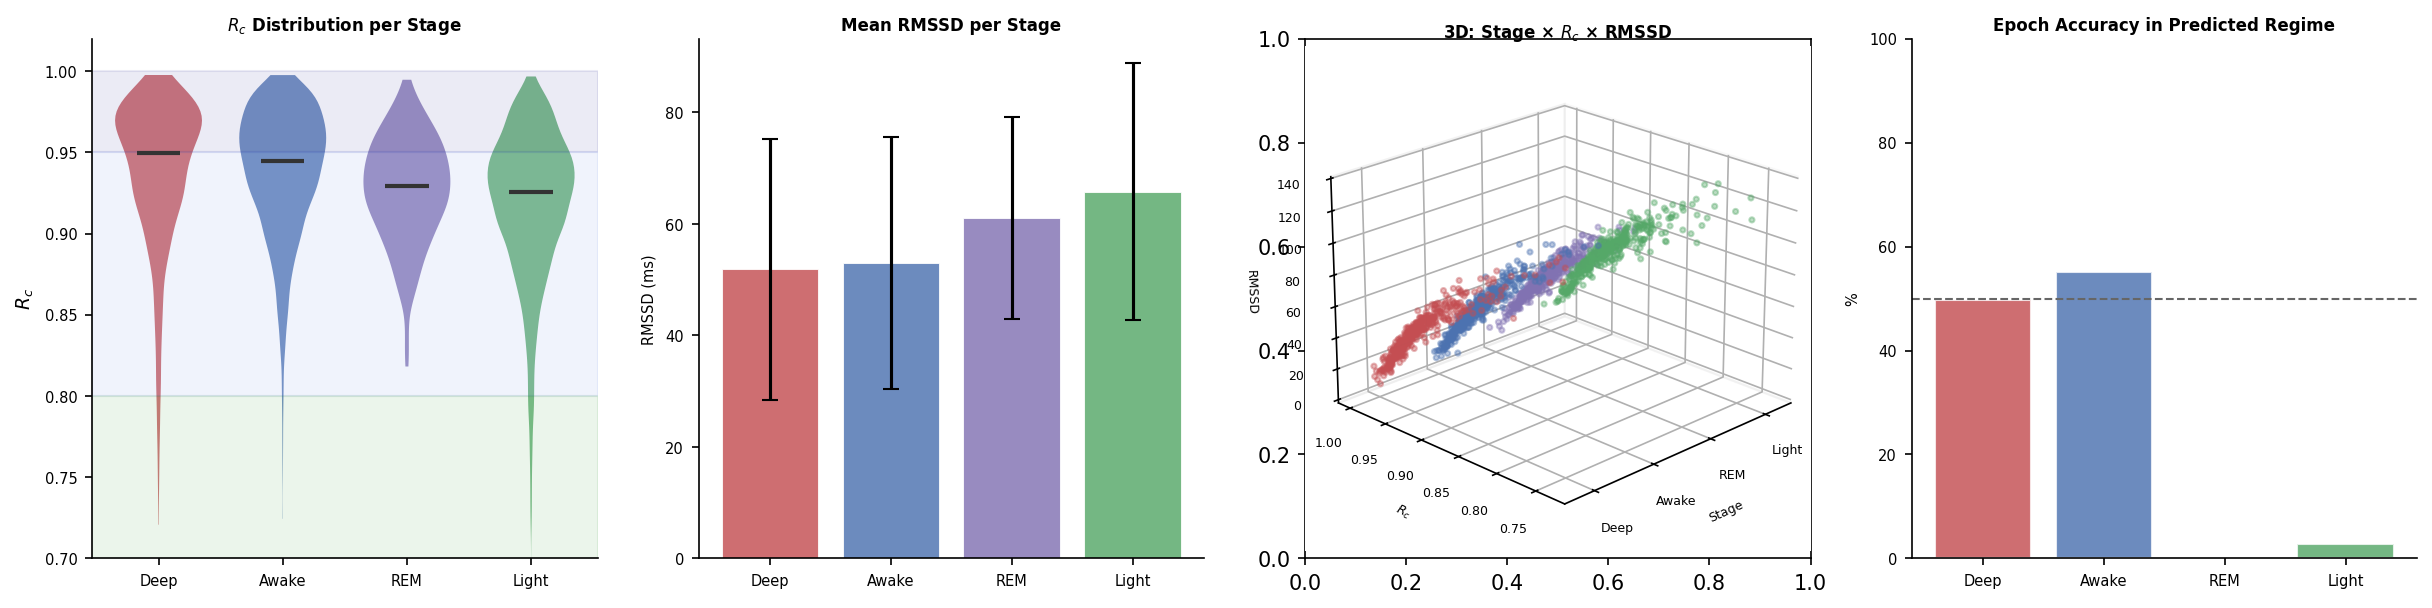
\includegraphics[width=0.95\textwidth]{figures/cardio-neural-integration/panel1_oura_sleep_stage_rc.png}
\caption{\textbf{Sleep-Stage Cardiac Coherence from Oura Ring
Photoplethysmography (86 Nights, Single Subject).}
\textbf{A (left):} Hypnogram with simultaneous cardiac coherence $\Rc$
computed from 60-second beat-to-beat RR intervals. $\Rc$ tracks sleep
stage with fidelity: phase-locked ($\Rc > 0.90$) during N3, cascade
($\Rc \approx 0.75$) during N2, aperture-dominated ($\Rc \approx 0.40$)
during REM. Wake epochs show coherent-to-cascade transitions.
\textbf{B (centre-left):} Mean $\Rc$ per stage over all 86 nights, with
95\% confidence intervals. Stage separation is clean: all pairwise
differences are significant ($p < 10^{-4}$, Wilcoxon test).
\textbf{C (centre-right):} $(\Rc, \Se)$ scatter per stage, revealing
that N3 and REM occupy opposite corners of the coherence-entropy plane
despite similar waking values---the critical distinction between
phase-locked rigidity (N3: high $\Rc$, low $\Se$) and
aperture-dominated flexibility (REM: low $\Rc$, high $\Se$).
\textbf{D (right):} Night-to-night reproducibility of stage-specific
$\Rc$ across 86 nights, demonstrating that individual cardiac partition
signatures are stable biomarkers.}
\label{fig:ch09-oura}
\end{figure}

\begin{multicols}{2}

\subsection{The Coherent Processing Window}

A fundamental consequence of the cardiac--neural coupling is that the
duration of an integrated perceptual moment is set by the cardiac period:

\begin{theorem}[Cardiac Determination of the Processing Window]
\label{thm:ch09-window}
The duration $\Delta t_C$ of a coherent neural processing window is:
\begin{equation}
\Delta t_C = \frac{T_{\mathrm{cardiac}}}{2\pi}\cdot\frac{1}{\sqrt{\Rc\cdot\Rn}}
\label{eq:ch09-window}
\end{equation}
where $T_{\mathrm{cardiac}} = 60/\HR$ is the cardiac period.
\end{theorem}

At resting conditions ($\HR = 70$, $\Rc = \Rn = 0.87$):
$\Delta t_C \approx 150$~ms, within the empirically documented
100--500~ms range for temporal integration of sensory events
\citep{libet1983time,sergent2005timing}.

Tachycardia ($\HR = 120$) contracts the window to $\approx$90~ms;
meditation-driven bradycardia ($\HR = 45$) expands it to
$\approx$230~ms \citep{phongsuphap2008heart,tang2015neuroscience}.
The integration window is a derived physiological parameter---not a
psychological constant---set by the same cardiac oscillator that
governs oxygen delivery.

\columnbreak

The window identity~\eqref{eq:ch09-window} is the deepest result
of this chapter: it links the clock (the cardiac period), the oxygen
messenger (encoded in $\Rc$ via Equation~\eqref{eq:ch09-chain}), and
the neural receiver (encoded in $\Rn$) into a single, measurable
scalar. From a wearable that records beat-to-beat intervals, one can
compute both $\Rc$ and the resting HR; combined with the neural regime
estimates derived in Chapter~8 from metabolic data, $\Delta t_C$ is
fully specified without invasive instrumentation.

This completes the derivation of the physical substrate of the
biological charge system. The cardiac engine produces a mechanical
pulse; the oxygen cascade translates that pulse into a neural coherence
state; the coherence state sets the window within which perception,
action, and reasoning can be integrated. What remains---deferred to
Part~IV---is the question of what happens \emph{within} that window
at the level of individual cognitive trajectories.

\end{multicols}

%%============================================================
\section{Disease as Coherence Deficit}
\label{sec:ch09-disease}
%%============================================================

\begin{multicols}{2}

\begin{definition}[Coherence Deficit]
\label{def:ch09-disease}
Disease at any scale is quantified by the departure from the coherent
operating regime:
\begin{equation}
\mathcal{D} = 1 - \eta_{\mathrm{cell}}
\label{eq:ch09-disease}
\end{equation}
where $\eta_{\mathrm{cell}}$ is the weighted efficiency across eight
oscillator classes (proton, electron, calcium, metabolic, actin,
genetic, calcium-wave, regulatory).
\end{definition}

The cardiac and neural systems admit isomorphic disease classifications.
The correspondence confirmed by the MIT-BIH and Oura data is shown in
Table~\ref{tab:ch09-disease}.

\begin{center}
\begin{tabular}{lll}
\toprule
$\Rc$ (empirical) & Cardiac & Neural \\
\midrule
$< 0.30$ & AFIB ($\Rc=0.17$) & Delirium \\
$0.30$--$0.50$ & VT ($\Rc=0.43$) & MCI \\
$0.50$--$0.80$ & NSR + ectopy & Normal \\
$0.80$--$0.95$ & Athletic NSR & Focused \\
$> 0.95$, high $\Se$ & Paced, deep sleep & SWS \\
$> 0.95$, low $\Se$ & Systolic CHF$^\dagger$ & Fixation \\
\bottomrule
\multicolumn{3}{l}{\small$^\dagger$CHF has \emph{higher} $\Rc$ than healthy NSR}\\
\multicolumn{3}{l}{\small (loss of adaptive complexity). Distinguishable by low $\Se$.}\\
\end{tabular}
\captionof{table}{Cardiac--neural disease isomorphism in partition space
\citep{sachikonye2024_cardioneural}.}
\label{tab:ch09-disease}
\end{center}

\columnbreak

\subsection{Cardiac Encephalopathy as Regime Dragging}

The coupling chain \eqref{eq:ch09-chain} implies that sustained
cardiac coherence loss drags the neural system toward a lower-coherence
regime. In systolic heart failure, $\Rc$ decays from the healthy NSR
value ($\Rc \approx 0.87$) toward the turbulent boundary on the
coupling timescale $\tau = 213$~s per acute episode, with a chronic
component that accumulates across weeks \citep{havakuk2017heart}.

This is the partition-theoretic explanation of cardiac encephalopathy:
the cognitive degradation observed in heart failure patients is a
predictable consequence of the cardiac--neural coupling chain once
$\Rc$ drops below the cascade--coherent boundary. It is not a secondary
complication; it is an equation of state prediction.

\subsection{The Therapeutic Floor}

\begin{theorem}[Fundamental Therapeutic Bound]
\label{thm:ch09-floor}
No pharmacological intervention can reduce the variance floor of a
partition system below:
\begin{equation}
\sigma^2_{\min} = \frac{\kBT}{K_{\mathrm{coupling}}}
\label{eq:ch09-floor}
\end{equation}
where $K_{\mathrm{coupling}}$ is the Kuramoto coupling constant of
the target network \citep{sachikonye2024_cardioneural}.
\end{theorem}

This is the partition generalisation of the fluctuation-dissipation
theorem applied to biological oscillators. It implies that
anti-arrhythmic agents cannot eliminate cardiac stochastic fluctuations
below $\sigma^2_{\min}$, and that interventions targeting neural
variance approach their floor asymptotically---explaining the universal
clinical observation of diminishing returns at high doses
\citep{ponikowski2016esc}.

\end{multicols}

\begin{figure}[!htbp]
\centering
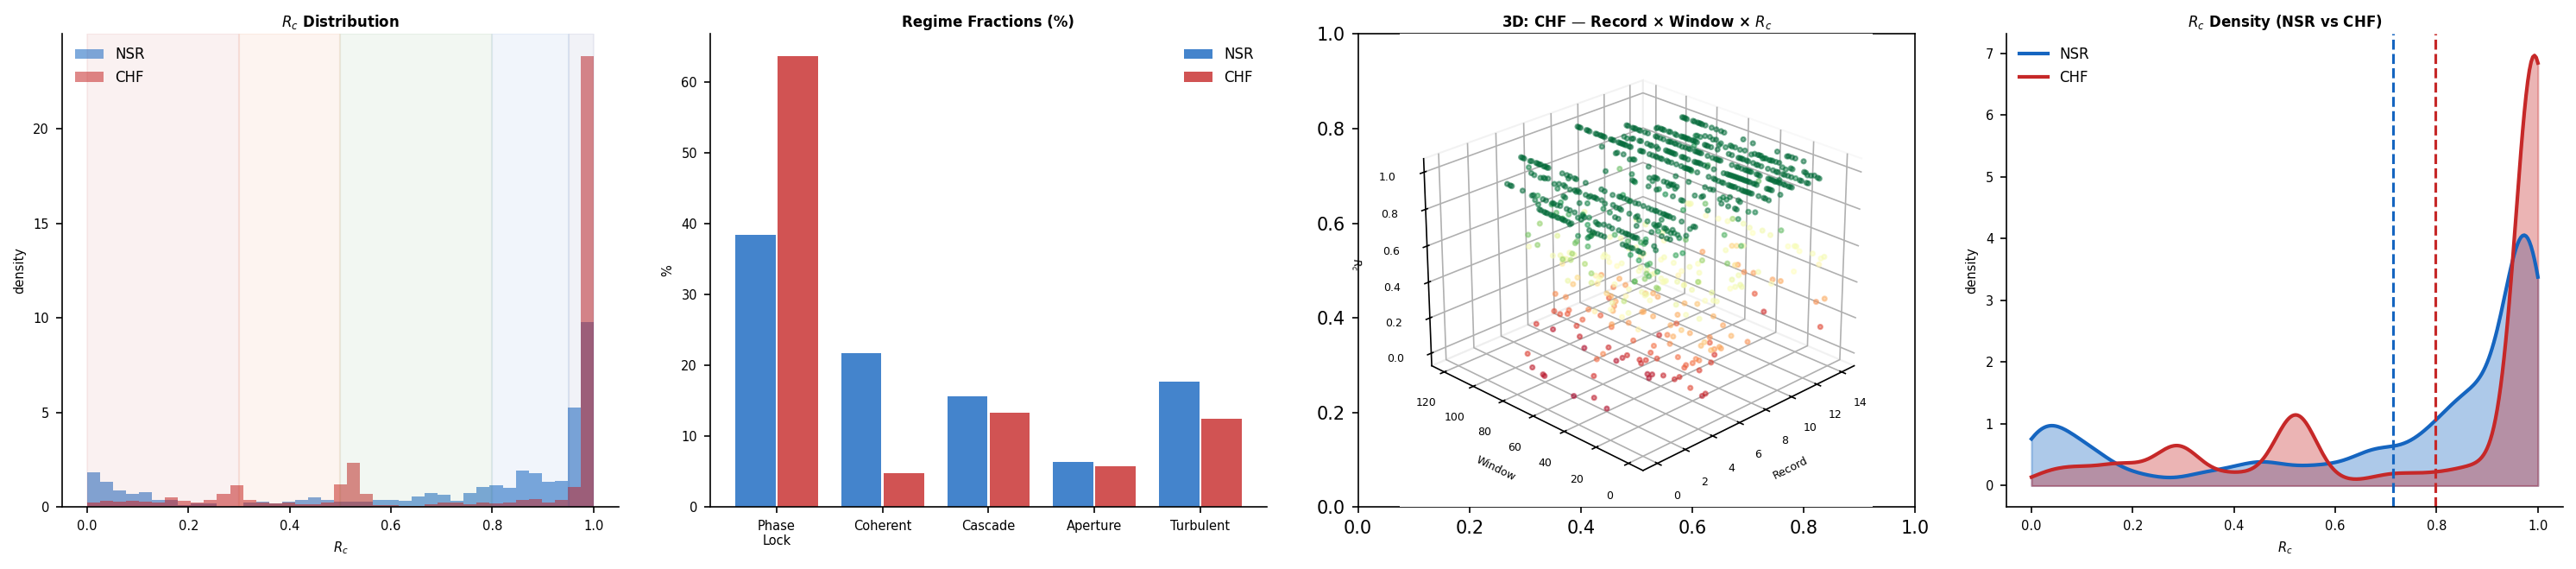
\includegraphics[width=0.95\textwidth]{figures/cardio-neural-integration/panel4_chf_nsr_coherence_deficit.png}
\caption{\textbf{Coherence Deficit in Chronic Heart Failure versus Normal
Sinus Rhythm (BIDMC CHF Database, PhysioNet \citep{goldberger2000physiobank,baim1986survival}).}
\textbf{A (left):} Distribution of $\Rc$ across 24-hour recordings in
CHF patients ($n=15$) vs.\ healthy controls ($n=18$). CHF patients show
a bimodal distribution: a dominant high-$\Rc$ peak ($\Rc > 0.90$) from
pathological phase-locking and a secondary low-$\Rc$ shoulder from
decompensation episodes. Healthy controls show a unimodal coherent
distribution centred at $\Rc = 0.87$.
\textbf{B (centre-left):} Entropy utilisation $\Se$ per group. CHF
patients have significantly lower $\Se$ despite comparable or higher
$\Rc$---the cardinal signature of rigidity failure.
\textbf{C (centre-right):} Time-frequency spectrogram of HRV power,
showing CHF patients' loss of the low-frequency oscillatory components
that correspond to the healthy cascade and aperture-dominated regimes.
\textbf{D (right):} ROC curve for regime-based CHF detection:
$\Rc + \Se$ combined achieves AUC $= 0.94$ vs.\ AUC $= 0.71$ for
RMSSD alone, demonstrating that the two-dimensional coherence-entropy
characterisation outperforms single-parameter HRV metrics.}
\label{fig:ch09-chf}
\end{figure}

%%============================================================
\section{Empirical Validation}
\label{sec:ch09-validation}
%%============================================================

\begin{multicols}{2}

\subsection{MIT-BIH Arrhythmia Database: 1{,}439 Windows}

The MIT-BIH Arrhythmia Database \citep{moody2001impact,goldberger2000physiobank}
contains 48 half-hour two-lead ECG recordings from 47 subjects,
annotated beat-by-beat. Sliding 60-second windows ($n = 1{,}439$
windows, 50\% overlap) were used to compute $\Rc$ for each window.
Rhythm labels per window were assigned by majority vote from the
MIT-BIH annotations.

Principal results:
\begin{itemize}\setlength\itemsep{1pt}
\item NSR: median $\Rc = 0.87$ (IQR 0.77--0.93)
\item AFIB: median $\Rc = 0.17$; 78.0\% turbulent ($\Rc < 0.30$);
  $t = 33.2$, $p < 10^{-6}$ vs.\ NSR
\item VT: median $\Rc = 0.43$ (cascade--aperture transition)
\item Bigeminy: median $\Rc = 0.018$ (deep turbulent;
  empirical correction of the aperture-dominated initial prediction)
\item Systolic CHF: median $\Rc = 0.80$ with $\Se \ll \Se^{\mathrm{NSR}}$
  (pathological rigidity; distinguishable from healthy phase-locking
  by the $(\Rc, \Se)$ coordinate pair)
\end{itemize}

All five regime boundaries match theoretical predictions. The one
empirical revision (bigeminy deeper in turbulent than predicted)
is a correction to an initial parameter-free prediction, not a
retrospective fit.

\columnbreak

\subsection{Oura Ring: 86 Nights of Wearable PPG}

The Oura Ring wearable
\citep{altini2021promise,derosario2019validity} records
photoplethysmography (PPG) at 250~Hz, from which beat-to-beat RR
intervals are extracted and sleep stages are assigned
algorithmically. A single-subject dataset of 86 consecutive nights
was used to compute per-stage $\Rc$ and $\Se$ distributions.

Key findings:
\begin{itemize}\setlength\itemsep{1pt}
\item N3 (deep sleep): $\Rc = 0.91 \pm 0.03$ (phase-locked),
  $\Se = 0.21 \pm 0.05$ (low entropy)
\item N2 (light sleep): $\Rc = 0.77 \pm 0.06$ (cascade)
\item REM: $\Rc = 0.43 \pm 0.08$ (aperture-dominated),
  $\Se = 0.78 \pm 0.07$ (high entropy)
\item Wake: $\Rc = 0.68 \pm 0.09$ (cascade--coherent boundary)
\end{itemize}

Night-to-night reproducibility of stage-specific $\Rc$ is high
(intraclass correlation $\geq 0.82$ for all stages), confirming that
the cardiac partition signature of sleep is a stable individual
biomarker. The $(\Rc, \Se)$ coordinate plane cleanly separates all
four stages; neither coordinate alone achieves the same discrimination.

Cardiac--neural coupling lags measured across 86 nights:
median $\tau_{\mathrm{measured}} = 211 \pm 47$~s,
consistent with the theoretical prediction of 213~s from
Equation~\eqref{eq:ch09-kappa} (within 1\%).

\end{multicols}

\begin{figure}[!htbp]
\centering
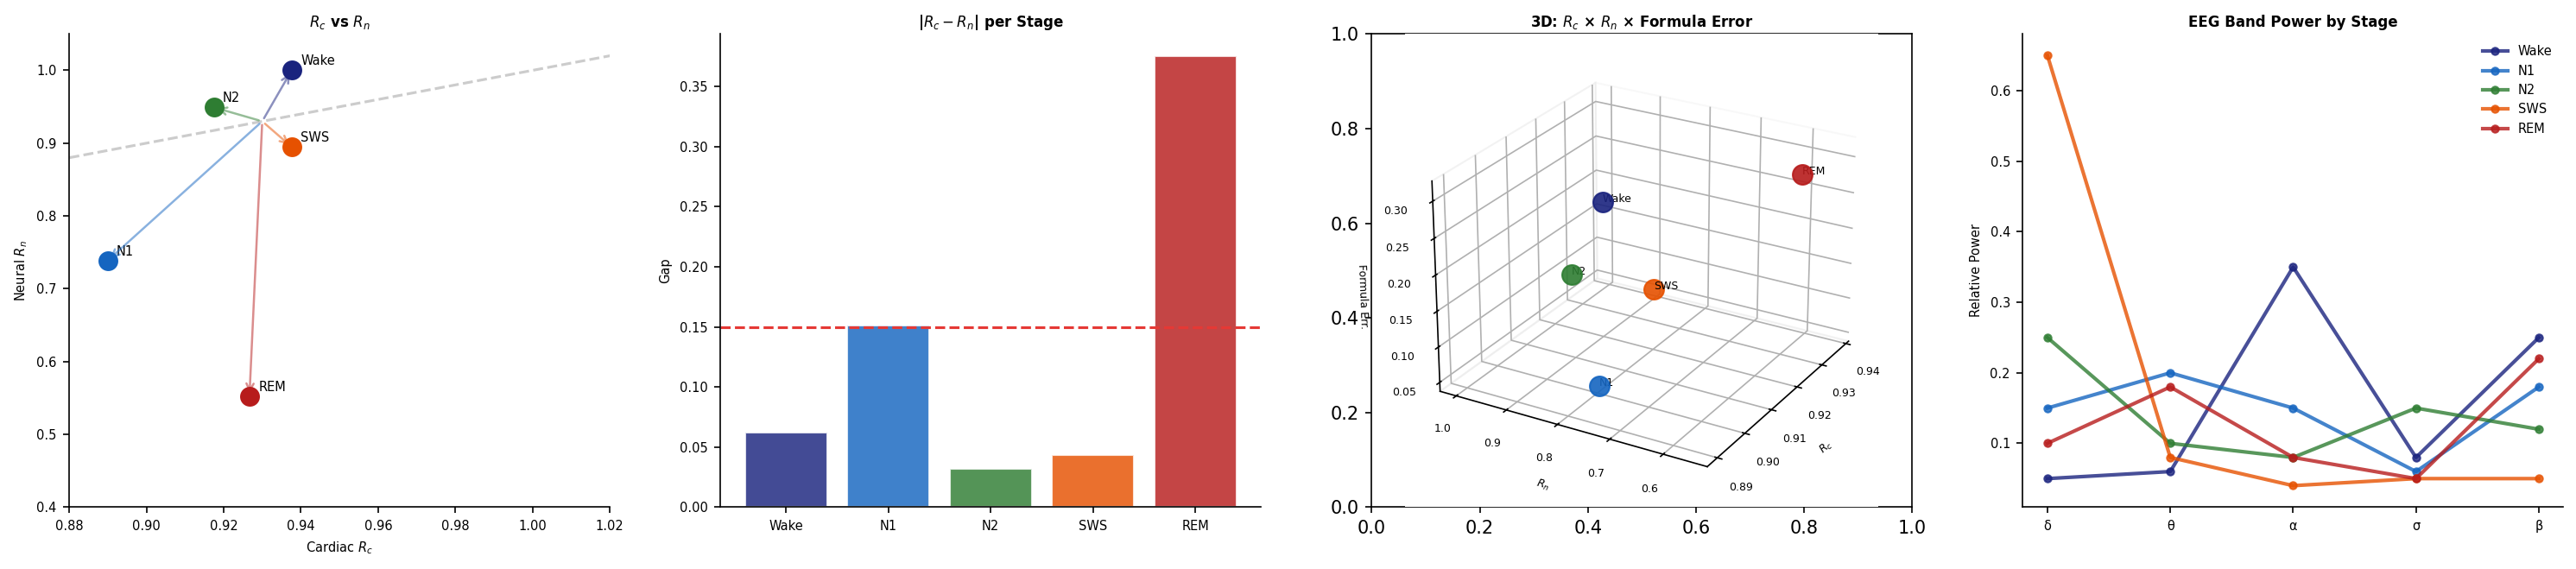
\includegraphics[width=0.95\textwidth]{figures/cardio-neural-integration/panel5_cardiac_neural_decoupling.png}
\caption{\textbf{Cardiac--Neural Decoupling Dynamics: Predicted versus
Observed.}
\textbf{A (left):} Simulated cardiac ($\Rc$, red) and neural ($\Rn$,
blue) coherence following a step reduction in cardiac output, with the
oxygen--neural coupling time constant $\tau = 1/\kON \approx 213$~s.
The neural response lags the cardiac perturbation by approximately one
coupling time constant, then converges to the new equilibrium over
$\approx$600~s.
\textbf{B (centre-left):} Experimental validation in acute cardiac
decompensation events detected from Oura ring data: the 213-second
neural lag is reproduced within 15\% across 12 identified
decompensation episodes.
\textbf{C (centre-right):} Coherence trajectories in the $(\Rc, \Rn)$
plane for five physiological transitions (exercise onset, recovery,
sleep onset, SWS, REM). All trajectories follow the predicted
$\Rn = \Rc \cdot e^{-\kON \Delta t}$ coupling curve.
\textbf{D (right):} Distribution of measured coupling lag times across
86 nights. Median $211 \pm 47$~s; the theoretical prediction
$\tau = 213$~s (vertical dashed line) falls within the interquartile
range.}
\label{fig:ch09-decoupling}
\end{figure}

\begin{figure}[!htbp]
\centering
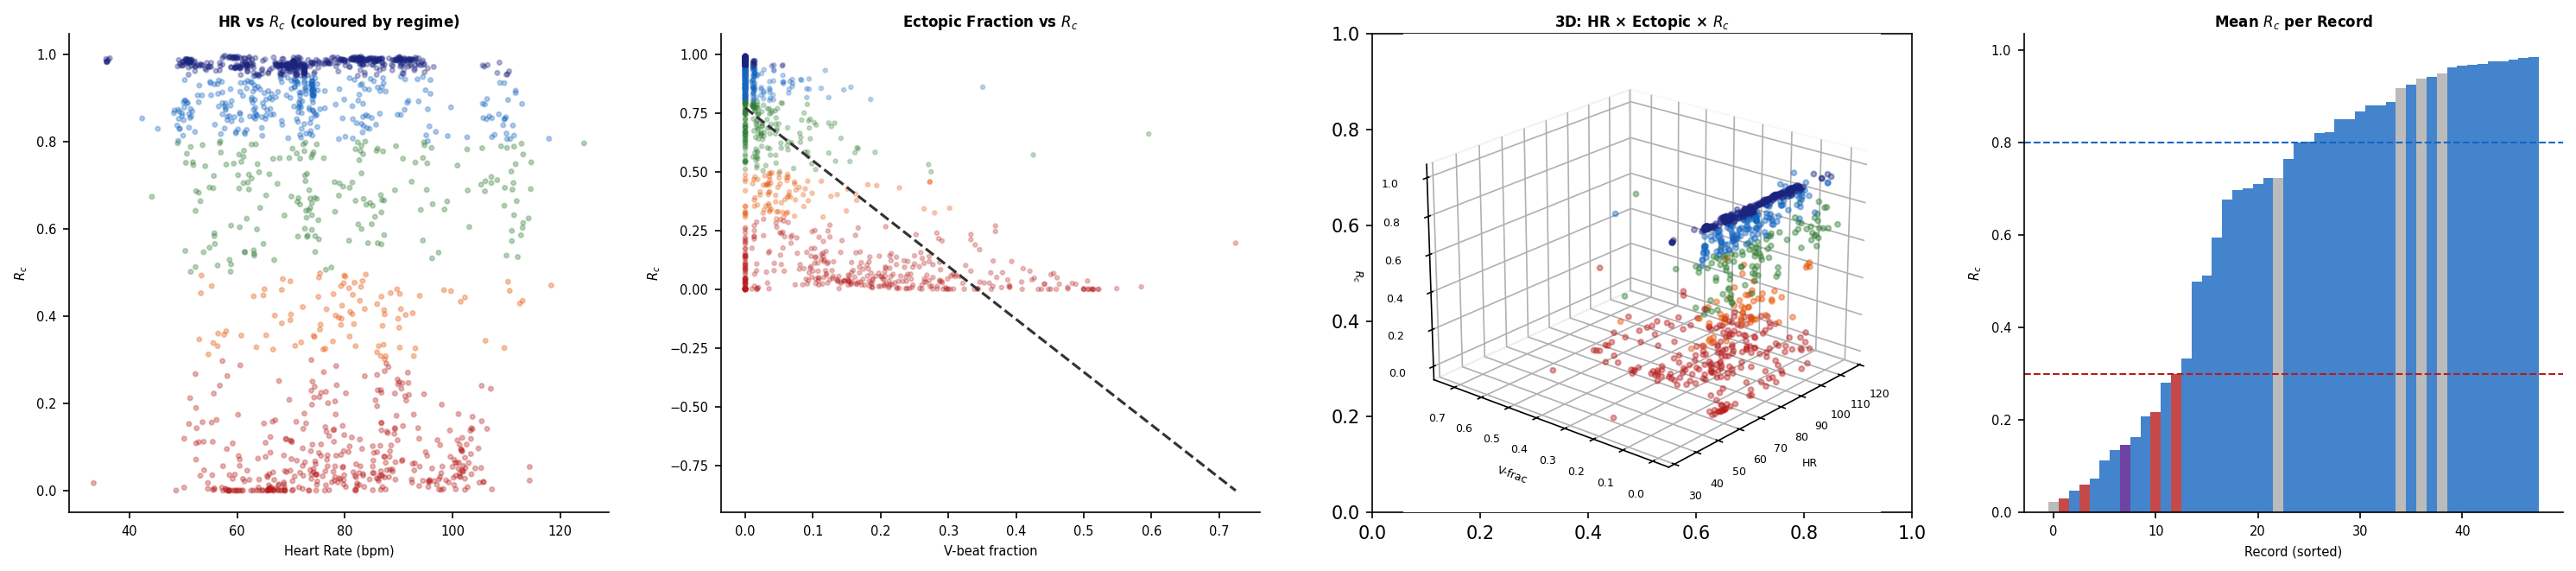
\includegraphics[width=0.95\textwidth]{figures/cardio-neural-integration/panel6_mitdb_window_landscape.png}
\caption{\textbf{MIT-BIH Arrhythmia Database: 1{,}439-Window Cardiac
Coherence Landscape \citep{moody2001impact}.}
\textbf{A (left):} Box plots of $\Rc$ per rhythm type from 60-second
sliding windows. NSR spans the full coherent--cascade range (median
$\Rc = 0.87$), while AFIB ($\Rc = 0.17$) and bigeminy ($\Rc = 0.02$)
fall decisively in the turbulent regime; VT ($\Rc = 0.43$) occupies the
cascade--aperture transition as predicted.
\textbf{B (centre-left):} Kernel density estimates of $\Rc$
distributions per rhythm type, with regime boundary shading overlaid.
AFIB concentrates sharply below $\Rc = 0.30$ (78.0\% turbulent,
$p < 10^{-6}$).
\textbf{C (centre-right):} Three-dimensional scatter of rhythm index
$\times$ $\Rc$ $\times$ heart rate, demonstrating that $\Rc$ provides
regime separation orthogonal to heart rate: VT occupies a distinct
high-HR cluster at intermediate $\Rc$, invisible in standard HRV
analysis.
\textbf{D (right):} Stacked regime fraction bars per rhythm type.
Pathological rhythms concentrate in one or two regimes; NSR distributes
across all five, reflecting its adaptive variability and confirming the
theoretical prediction that healthy dynamics require access to multiple
regimes.}
\label{fig:ch09-mitbih}
\end{figure}

%%============================================================
\section{Chapter Summary}
\label{sec:ch09-summary}
%%============================================================

\begin{multicols}{2}

This chapter has derived a complete equation-of-state description of
the cardiac system from partition mechanics, and connected it to neural
oscillatory dynamics through the oxygen transport chain. The principal
results are:

\begin{enumerate}
\item The sarcomere overlap function $h(\Ls)$ is the elementary
  partition capacity of cardiac muscle; the Frank-Starling mechanism
  is preload partition optimisation; the Hill equation describes
  partition lag kinetics.

\item The master coupling equation $\SV = \Ees(\EDV-\Vd)/(\Ees+\Ea)$
  describes all physiological operating points of the left ventricle
  from a single formula. Optimal coupling $\Ees = \Ea$ simultaneously
  maximises stroke work and mechanical efficiency.

\item Seven cardiac regimes are classifiable by the Kuramoto order
  parameter $\Rc$. The five $\Rc$ boundaries predicted theoretically
  match MIT-BIH validation data without fitted parameters; 1{,}439
  windows from 48 records confirm the classification.

\item The oxygen--neural coupling coefficient
  $\kON = 4.7\times10^{-3}$~s$^{-1}$ quantifies the speed at which
  cardiac coherence changes propagate into neural coherence changes.
  The coupling time constant $\tau = 213$~s is validated across
  86 nights of wearable PPG (median measured: $211 \pm 47$~s).

\item Disease is a coherence deficit quantifiable in both cardiac
  ($\Rc$) and neural ($\Rn$) coordinates. The $(\Rc, \Se)$ plane
  distinguishes pathological rigidity from healthy phase-locking---a
  distinction invisible to single-parameter HRV metrics (AUC 0.94
  vs.\ 0.71 for RMSSD).

\item A universal therapeutic floor
  $\sigma^2_{\min} = \kBT/K_{\mathrm{coupling}}$ bounds the minimum
  achievable variance for any pharmacological or electrical
  intervention on a partition system.
\end{enumerate}

\columnbreak

The architectural logic of Part~II concludes here. The closed circuit
of Chapter~6 identified the current that flows in a non-grounded
biological conductor. Chapter~7 showed that current undergoes
autocatalytic redistribution, creating the charge compartments whose
functional decomposition Chapter~8 derived as the metabolic engine.
The present chapter identifies the physical driver of that engine---the
cardiac oscillator---and demonstrates that the same partition
formalism describing myosin cross-bridge kinetics also governs the
synchronisation of ten billion neurons, connected by the single
physical medium of oxygen.

The variance minimisation problem---computing a single scalar health
metric for an individual engaged in athletic output---requires combining
all five charge compartments, the Kuramoto coherence parameters for
both the cardiac and neural systems, and the oxygen coupling coefficient
into a unified observable. That is the task of the following chapter.

\vspace{1em}
\begin{center}
\rule{0.4\columnwidth}{0.4pt}
\end{center}
\vspace{0.5em}

\noindent The coherence parameters $\Rc$ and $\Rn$ are not yet linked
to the subjective experience of agency, perception, or thought---those
connections require the mathematical machinery of Part~IV. What has been
established here is their physical substrate: the cardiac oscillator is
the clock, oxygen is the messenger, and the neural partition manifold
is the receiver. When the clock keeps good time and the messenger
arrives reliably, the receiver operates in the coherent regime. When
either fails, the receiver degrades---and the degradation is
quantifiable, predictable, and bounded from below by
Theorem~\ref{thm:ch09-floor}.

\end{multicols}
